\documentclass{article}
\usepackage[utf8]{inputenc}
\usepackage[ngerman]{babel}
\usepackage[T1]{fontenc}
\usepackage{lmodern}
\usepackage{graphicx}
\usepackage[locale=DE]{siunitx}
\usepackage{float}
\usepackage[nottoc,numbib]{tocbibind}
\newcommand{\RM}[1]{\MakeUppercase{\romannumeral #1}}


\usepackage{longtable}

\usepackage{bibgerm}

\usepackage{footnpag}

\usepackage{ifthen}

\usepackage{graphicx}

\usepackage{here}

\usepackage{amsmath}

\usepackage{amsxtra}

\usepackage{amsfonts}

\usepackage{amssymb}

\usepackage{url}

%Für Testzwecke aktivieren, zeigt labels und refs im Text an.

%\usepackage{showkeys}

% Abstand zwischen zwei Absätzen nach DIN (1,5 Zeilen)

\setlength{\parskip}{1.5ex plus0.5ex minus0.5ex}

% Einrückung am Anfang eines neuen Absatzes nach DIN (keine)

\setlength{\parindent}{0pt}

% Ränder definieren

\setlength{\oddsidemargin}{0.3cm}

\setlength{\textwidth}{15.6cm}

% bessere Bildunterschriften

\usepackage[center]{caption2}

% Problemlösungen beim Umgang mit Gleitumgebungen

\usepackage{float}

% Nummeriert bis zur Strukturstufe 3 (also <section>, <subsection> und <subsubsection>)

\setcounter{secnumdepth}{3}

% Führt das Inhaltsverzeichnis bis zur Strukturstufe 3

\setcounter{tocdepth}{3}

\usepackage{exscale}





% führt mit \vv zu längenangepassten vektorpfeilen

\usepackage{esvect}

%Ergibt eine nummerierte Aufzählung bei enumerate

%\begin{compactenum}[(i)] führt zu (i), (ii), (iii), (iv), ...

%\begin{compactenum}[(I)] führt zu (I), (II), (III), (IV), ...

%\begin{compactenum}[a)] führt zu a), b), c), d), ...

\usepackage{paralist}


\newenvironment{dsm} {\begin{displaymath}} {\end{displaymath}}

\newenvironment{vars} {\begin{center}\scriptsize} {\normalsize \end{center}}

\newcommand {\en} {\varepsilon_0} % Epsilon-Null aus der Elektrodynamik

\newcommand {\lap} {\; \mathbf{\Delta}} % Laplace-Operator

\newcommand {\R} { \mathbb{R} } % Menge der reellen Zahlen

\newcommand {\e} { \ \mathbf{e} } % Eulersche Zahl

\renewcommand {\i} { \mathbf{i} } % komplexe Zahl i

\newcommand {\N} { \mathbb{N} } % Menge der nat. Zahlen

\newcommand {\C} { \mathbb{C} } % Menge der kompl. Zahlen

\newcommand {\Z} { \mathbb{Z} } % Menge der kompl. Zahlen

\newcommand {\limi}[1]{\lim_{#1 \rightarrow \infty}} % Limes unendlich

\newcommand {\sumi}[1]{\sum_{#1=0}^\infty}

\newcommand {\rot} {\; \mathrm{rot} \,} % Rotation

\newcommand {\grad} {\; \mathrm{grad} \,} % Gradient

\newcommand {\dive} {\; \mathrm{div} \,} % Divergenz

\newcommand {\dx} {\; \mathrm{d} } % Differential d

\newcommand {\cotanh} {\; \mathrm{cotanh} \,} %Cotangenshyperbolicus

\newcommand {\asinh} {\; \mathrm{areasinh} \,} %Area-Sinus-Hyp.

\newcommand {\acosh} {\; \mathrm{areacosh} \,} %Area-Cosinus-H.

\newcommand {\atanh} {\; \mathrm{areatanh} \,} %Area Tangens-H.

\newcommand {\acoth} {\; \mathrm{areacoth} \,} % Area-cotangens

\newcommand {\Sp} {\; \mathrm{Sp} \,}

\newcommand {\mbe} {\stackrel{\text{!}}{=}} %Must Be Equal

\newcommand{\qed} { \hfll $\square$\\}

\renewcommand{\i} {\imath}

\newcommand{\ham}{\mathcal{H}}

\newcommand{\lag}{\mathcal{L}}

\def\captionsngerman{\def\figurename{\textbf{Abb.}}}

\renewcommand{\dagger}{**}

\renewcommand{\contentsname}{Inhaltsverzeichnis}

\renewcommand{\figurename}{Abbildung}

\renewcommand{\tablename}{Tabelle}

%\scriptsize \Large

\begin{document}
	\scriptsize \normalsize
	\title{ Tomographie mittels $\gamma$-Strahlung  \\ Versuch 14}
	

	
	\author{Polina Stecher\\ {polina.stecher@tu-dortmund.de}  \and   Ramona Gabrie\\ {sonya.djuffouo@tu-dortmund.de}} %{polina.stecher@tu-dortmund.de  sonya.djuffouo@tu-dortmund.de} 
	\date{Durchgeführt am  19. Juni  2018}
		\maketitle
	\newpage
	\tableofcontents
	\thispagestyle{empty}
	\newpage
	\newpage
	
\section{Zielsetzung und Motivation}
Ziel des Versuches ist es, die spezifische Molwärme von Kupfer in Abhängigkeit der Temperatur zu untersuchen. Desweiteren wird aus den gewonnenen Ergebnissen die sogenannte Debye-Temperautr $\Theta_D$ bestimmt und mit dem theoretischen Ansatz verglichen. Insgesamt existieren drei Modelle, die die Abhängigkeit der Molwärme und der Temperatur beschreiben. Zum einem gibt es die klassische Theorie, das Einsteins-Modell und das Debye-Modell.

\section{Theorie} 
\subsection{Die klassische Theorie der Molwärme}
Die klassische Betrachtung besagt, dass die thermische Energie, die in einen Körper eingebracht wird, sich gleichmäßig auf die Freiheitsgrade der Atome des Festkörpers verteilt. Die Atome sind durch Gitterkräfte an feste Plätze gebunden und können in drei Richtungen schwingen und haben somit drei Freiheitsgrade. Die Atome führen eine harmonische Schwingung um ihre Ruhelage aus und haben somit eine mittlere kinetische Energie, die mit der potentiellen Energie identisch ist. Die mittlere Energie eines Atoms beträgt
\begin{align}
E=6\dfrac{1}{2}k_BT
\end{align}
mit der Boltzmann-Konstante $k_B$  und der Temperatur T. In einem Kristall betrachtet, ergibt sich daraus mit der Loschmidt-Konstante $N_L$ (Teilchendichte eines idealen Gases)
\begin{align}
E=3k_bN_LT.
\end{align}
Unter Vorraussetzung eines konstanten Volumens folgt für die spezifische Wärmekapazität
\begin{align}
C_V=(\dfrac{\delta E}{\delta T})_V=3R.
\end{align}
Somit ist die spezifische Molwärme nach der Gleichung (3) material-und temperaturunabhängig. In der Realität trifft diese Annahme nur für hohe Temperaturen ($T\gg\Theta_D$) zu. 
\subsection{Die Einstein-Theorie}
Im Einsteinschen-Modell wird im Gegensatz zur klassischen Theorie die Quantelung der Schwingungsenergie der Atome berücksichtigt. Dabei wird angenommen, dass alle Atome im Festkörper jeweils mit der gleichen Frequenz $\omega$ schwingen und nur Energien von ganzzahligen Vielfachen des Wertes $\hbar\omega$ aufnehmem bzw. abgeben. Mittels der Boltzmannschen Wahrscheinlichkeitsverteilung 
\begin{align}
W(n)=exp(\dfrac{-n\hbar \omega}{k_BT})
\end{align}
wird die Wahrscheinlichkeit eines sich im thermischen Gleichgewicht befindenen Oszillators mit der Energie $n\hbar\omega$ bei einer Temperatur T angegeben. Aus der Verteilung ergibt sich die Einstein-Energie
\begin{align}
E_{Einstein}=\dfrac{\hbar\omega}{e^{\dfrac{\hbar \omega}{k_BT}}-1}.
\end{align}
Die Molwärme berechnet sich somit zu 
\begin{align}
C_V=3R\left(\dfrac{\hbar\omega}{k_B}\right)^2 \dfrac{1}{T^2} \dfrac{exp(\dfrac{\hbar\omega}{k_BT})}{(exp(\dfrac{\hbar \omega}{k_BT})-1)^2}
\end{align}
mit der Einstein-Temperatur $\Theta_E=\dfrac{\hbar \omega_E}{k_BT}$. Auch bei diesem Modell gilt eine Annäherung an 3R bei sehr hohen Temperaturen. 
\subsection{Debye-Modell}
Zu den Modellen, die das Verhalten der Abhängigkeit der Molwärme und der Temperatur am nähesten beschreibt, zählt das Debye-Modell. Das Modell basiert darauf, dass die Eigenschwingung aller Oszillatoren in einem Festkörper eine spektrale Frequenzverteilung $Z(\omega)$ mit der  Grenzfrequenz $\omega_D$ besitzt. Bis zur Grenzfrequenz ist die lineare Dispersionsrelation (Frequenz und Wellenvektor proportional) gegeben. Durch Verknüpfen von klassischem und quantenmechanischem Modell, ergibt sich eine Näherung mit der Form für die spektrale Verteilung von 
\begin{align}
Z(\omega)d\omega=\dfrac{L^3}{2\pi^2}\omega^2\left(\dfrac{1}{v_{long}^3}+\dfrac{2}{v_{trans}^3}\right)d\omega.
\end{align}
Mit der Debye-Grenzfrequenz wird diese Gleichung zu 
\begin{align}
Z(\omega)d\omega=\dfrac{9N_L}{\omega_D^3}\omega^2 d\omega.
\end{align}
Damit kann die Molwärme im Debye-Modell berechnet werden über
\begin{align}
C_{V,Debye}=\dfrac{d}{dT}\dfrac{9N_L}{\omega_D^3}\int_{0}^{\omega_D}\dfrac{\omega^3}{exp(\hbar\omega/k_BT)-1}.
\end{align}
Wie bei den anderen Modellen, nähert sich auch die Debye Kurve im hohen Temperatur Bereich dem Wert 3R an. 

\subsection{Vergleich der drei Modelle}
In der Abbildung (1) werden die Verläufe der drei Modelle mit dem experimentellem Befund verglichen. Zunächst ist zu erkennen, dass für hohe Temperaturen (ab 300 K) das Einstein- und das Debye Modell sich dem Wert von 3R annähern. Für niedrige Temperaturen (0-300K) hingegen nimmt der Verlauf der speziellen Molwärme nach Einstein exponentiell mit der Temperatur zu, wohingegen es bei dem Debye-Modell eine $T^3$-Abhängikeit für tiefe Temperaturen gibt. Anhand der Abbildung lässt sich erkennen, dass das Debye-Modell sich dem experimentellen Verlauf am meisten nähert. 
\begin{figure}[H]
	\centering
	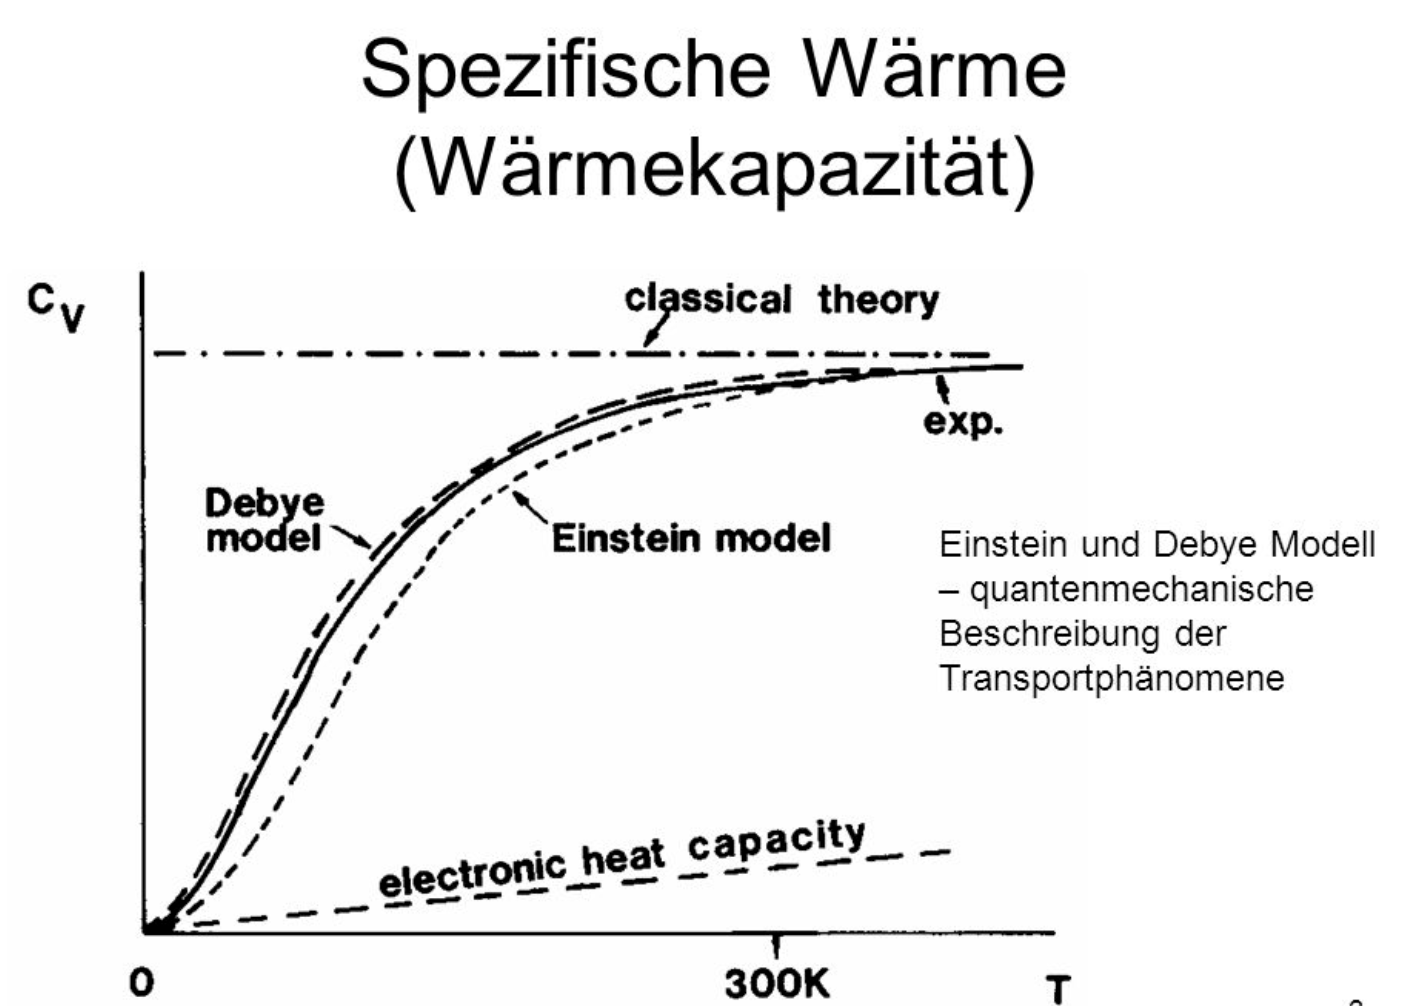
\includegraphics[height=7cm, width=10cm]{vergleich.png}
	\caption{  Vergleich der drei Graphiken von der klassichen Theorie, des Einstein-Modells und des Debye-Modells$^{[2]}$}   
	\label{fig: abb. 1}
\end{figure} 
\section{Versuchsaufbau und Durchführung}
\subsection{Versuchsaufbau}
Die Abbildung (2) zeigt die Apparatur, die zur Bestimmung der Molwärme von Kupfer verwendet wurde. 

\begin{figure}[H]
	\centering
	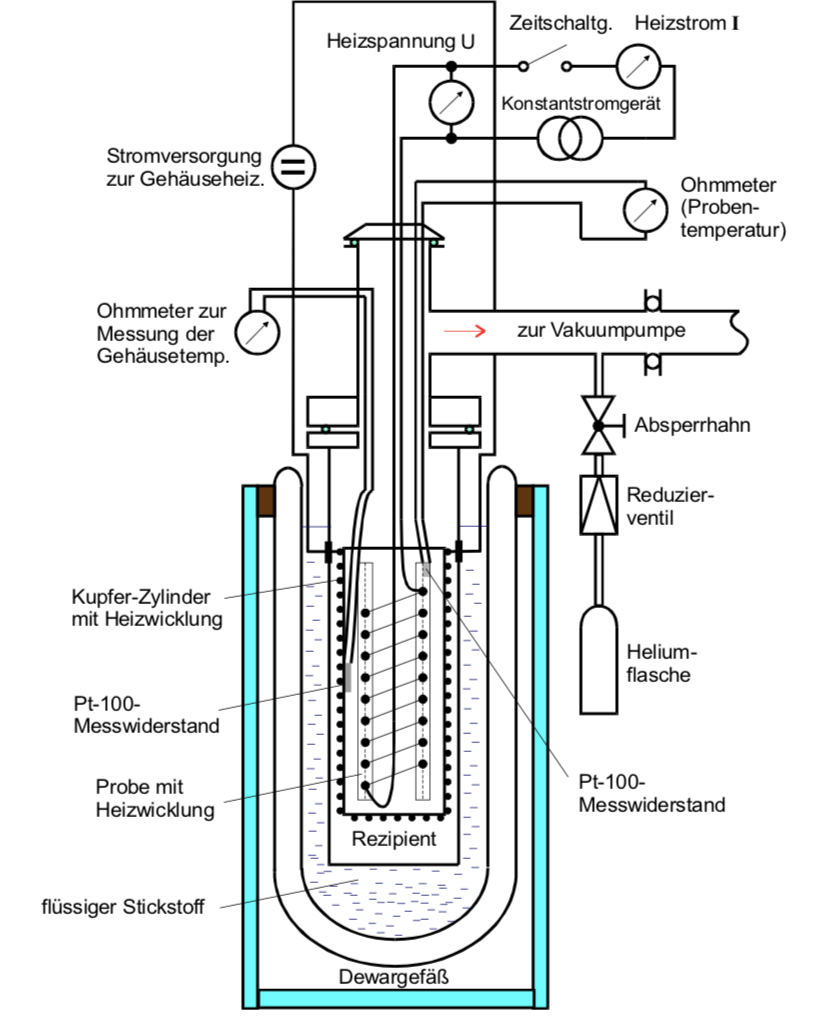
\includegraphics[height=10cm, width=8cm]{aufbau.png}
	\caption{ Versuchsapparatur $^{[1]}$}   
	\label{fig: abb. 1}
\end{figure}
Der Versuchsaufbau besteht aus einem Dewar-Gefäß. In dieses Gefäß wird im Laufe des Experiments flüssiges Stickstoff gefüllt. Im Inneren des Gefäßes befindet sich das Rezipient, in dem die Kupferprobe eingelagert ist. Diese Kupferprobe besitzt eine eigene Heizwicklung, welche ihrerseits von einem Kupfer-Zylinder mit Heizwicklung umgeben ist. An der Probe und dem Zylinder sind jeweils ein PT-100 Messwiderstand befestigt, der zur Bestimmung der Temperatur benötigt wird. Weiterhin ist der Rezipient an einer Vakuumpumpe und Heliumflasche angeschlossen ist. Die Erhitzung der Probe und des Zylinders erfolgen über die verbundene Stromversorgung und Heizspannung U. 
\subsection{Durchführung}
Zunächst wird das Rezipient evakuiert, damit kein Wärmeverlust durch die Konvektion über die Gasmoleküle geschieht. Anschließend wird Helium bei Barometerdruck in den Rezipient gefüllt und mit Hilfe des flüssigen Stickstoffs im Dewar Gefäß wird die Probe auf 80 K abgekühlt. Helium eignet sich deshalb so gut, weil es einen niedrigeren Schmelzpunkt als Luft besitzt und sich bei der Abkühlung nicht verflüssigt im Gegensatz zu Luft. Nach ca. einer Stunde ist die Endtemperatur erreicht und das Rezipient wird evakuiert, um den Innendruck zu veringern. Anschließend wird der abgekühlten Probe elektrische Energie über die Heizwicklung zugeführt. Die Temperaturerhöhung $\Delta T$ wird über die Widerstände gemessen. Der Kupfer-Zylinder sollte während des gesamten Versuches die gleiche Temperatur wie die Probe aufweisen, um so den Wärmeverlust aufgrund der Wärmübertragung durch einen Temperaturgradienten zu verhindern. Um dies zu ermöglichen, ist der Kupfer Zylinder an eigener Stromversorgung angeschlossen, damit elektrische Energie zugeführt werden kann. Ziel der Messung ist es die Molwärme von Kupfer für verschiedene Temperaturen zwischen 80 bis 300 Kelvin zu ermitteln. Dazu wird die Probe im Zeitabstand von fünf Minuten regelmäßig über die Stromstärke erhitzt. Währenddessen wird die Temperatur, die Messzeit, die Spannung und der Heizstrom bei konstantem Volumen notiert. 
\end{document}